\begin{figure}[ht]
\centering
% Thesis-wide categorical color palette
% Usage: % Thesis-wide categorical color palette
% Usage: % Thesis-wide categorical color palette
% Usage: \input{figures/palette} in any figure file
%
% Muted primary colors -- print-friendly, visually distinct.
% Inspired by Cooper Union's red/blue primaries, softened for
% academic figures. Use palA-palC for data series in scatter
% plots, line charts, bar charts, etc.

\definecolor{palA}{HTML}{1F77B4}   % Tableau blue
\definecolor{palB}{HTML}{D62728}   % Tableau red
\definecolor{palC}{HTML}{2CA02C}   % Tableau green
 in any figure file
%
% Muted primary colors -- print-friendly, visually distinct.
% Inspired by Cooper Union's red/blue primaries, softened for
% academic figures. Use palA-palC for data series in scatter
% plots, line charts, bar charts, etc.

\definecolor{palA}{HTML}{1F77B4}   % Tableau blue
\definecolor{palB}{HTML}{D62728}   % Tableau red
\definecolor{palC}{HTML}{2CA02C}   % Tableau green
 in any figure file
%
% Muted primary colors -- print-friendly, visually distinct.
% Inspired by Cooper Union's red/blue primaries, softened for
% academic figures. Use palA-palC for data series in scatter
% plots, line charts, bar charts, etc.

\definecolor{palA}{HTML}{1F77B4}   % Tableau blue
\definecolor{palB}{HTML}{D62728}   % Tableau red
\definecolor{palC}{HTML}{2CA02C}   % Tableau green

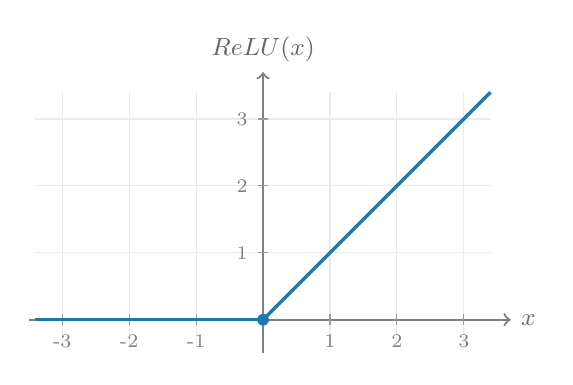
\begin{tikzpicture}[
    scale=0.85,
]

% Grid
\draw[black!8, step=1] (-3.4, -0.4) grid (3.4, 3.4);

% Axes
\draw[->, black!50, thick] (-3.5, 0) -- (3.7, 0)
    node[right, font=\small, text=black!60] {$x$};
\draw[->, black!50, thick] (0, -0.5) -- (0, 3.7)
    node[above, font=\small, text=black!60] {$\text{ReLU}(x)$};

% Tick marks
\foreach \x in {-3,-2,-1,1,2,3} {
    \draw[black!40] (\x, -0.08) -- (\x, 0.08);
    \node[font=\scriptsize, text=black!50, below=2pt] at (\x, 0) {\x};
}
\foreach \y in {1,2,3} {
    \draw[black!40] (-0.08, \y) -- (0.08, \y);
    \node[font=\scriptsize, text=black!50, left=2pt] at (0, \y) {\y};
}

% ReLU function
\draw[palA, very thick] (-3.4, 0) -- (0, 0);
\draw[palA, very thick] (0, 0) -- (3.4, 3.4);

% Kink marker
\fill[palA] (0, 0) circle (2.5pt);

\end{tikzpicture}
\caption{The ReLU activation function: negative inputs are zeroed,
  positive inputs pass through unchanged.}
\label{fig:relu}
\end{figure}
